\section{Various}


\subsection{Two-Sampled t-Test}

\subsubsection{Unpaired Data}

We have $X_i$ i.i.d. $\sim \mathcal N(\mu_X, \sigma^2)$ and $Y_j$ i.i.d. $\sim \mathcal N(\mu_Y, \sigma^2)$ with $X_i, Y_j$ independent. For the $t$-test, $H_0: \mu_X = \mu_Y$ and $H_A: \mu_X \neq \mu_Y$. Then:
$$T = \frac{\bar X_n - \bar Y_m}{\sqrt{\frac{s^2}{n} + \frac{s^2}{m}}} \sim t_{n+m-2} \text{ under } H_0$$

\subsubsection{Paired Data}

We have independent $D_i = X_i - Y_i$ and:
$$\bar D = \frac{1}{n} \sum_{i=1}^n D_i \sim \mathcal N(\mu_D, \sigma_D / \sqrt{n})$$

$H_0$ and $H_A$ as before and:
$$T = \sqrt{n} \frac{\bar D}{S_D} \sim t_{n-1} \text{ under } H_0$$

\subsection{Charts}

\begin{lstlisting}
stripchart(y ~ x, vertical = T, pch = 1, data = d)
boxplot(y ~ x, data = d)
with(d, interaction.plot(x.factor = a, trace.factor = b, response = y))
\end{lstlisting}


\subsection{Data Generation / Calculations}
\begin{lstlisting}
## Generate 10 A's followed by 10 B's
rep(c("A", "B"), each = 10)

## Alternate A, B 10 times
rep(c("A", "B"), times = 10)

## Toss a coin 20 times (1/2 prob. for A, B)
sample(c("A", "B"), 20, replace = T)

## Choose 10 A's at random, the rest B's
sample(rep(c("A", "B"), times = 10), 20, replace = F)

## Overall mean of column A
mean(d$A) ## or aggreagte(A ~ 1, data = d, mean)

## Group mean per B
aggregate(A ~ B, data = d, mean)
\end{lstlisting}


\subsection{Examples}

\subsubsection{Split-Plot Design, ANOVA Skeleton}

Three new types of pizzas in six different packings are investigated by 90 consumers on a 0-10 scale. Each person rates the six packings of just one type of pizza, that is pizzas are randomized to persons and each person tastes the different packings in random order. \medskip

This is a split-plot design with persons as whole plots and rating orders (or time slots) as split plots. Pizza type is the whole-plot factor, packing the split-plot factor. We have:
$$Y_{ijk} = \mu + \beta_i + \eta_{k(i)} + \alpha_j + (\alpha \beta)_{ij} + \epsilon_{k(ij)}$$

Where $\eta_{k(i)}$ is the whole-plot error. The ANOVA skeleton is given by:
\begin{center}
	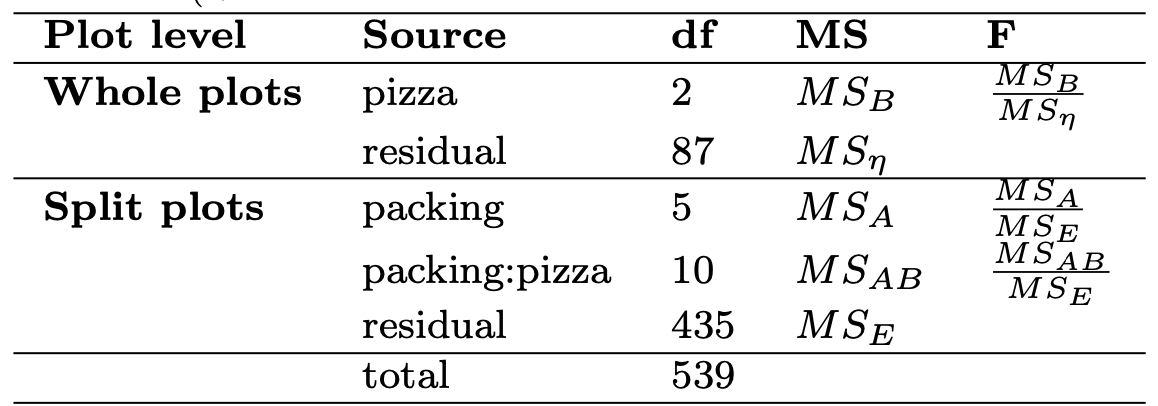
\includegraphics[width=\linewidth]{anova-skeleton.png}
\end{center}

\subsubsection{Split-Plot Design with Blocking}

A soil scientist wanted to investigate the effects of nitrogen supplied in four different forms and later evaluate those effects combined with those of thatch accumulation (two, five or eight years of accumulation) on the quality of an established turf. A golf green had been constructed and seeded with grass on the experimental plots. The nitrogen treatment plots were arranged on the golf green in a randomized complete block design with two block levels. Each of the eight experimental plots was split into three subplots to which the levels of the second treatment factor were randomly assigned. \medskip

This is a split-plot design with whole-plot factor nitrogen, split-plot factor thatch and a block factor block.
$$Y_{ijkl} = \mu + \gamma_i + \alpha_j + \beta_k + (\alpha \beta)_{jk} + \eta_{l(ij)} + \epsilon_{l(ijk)}$$

Where $l = 1$, $\gamma_i$ fixed effect of the block, $\alpha_j$ fixed main effect of nitrogen, $\beta_k$ fixed main effect of thatch, $(\alpha \beta)_{jk}$ interaction, $\eta_{l(ij)}$ error on the whole-plot level and $\epsilon_{l(ijk)}$ the error on the split-plot level.

